\documentclass{article}
\usepackage{graphicx} % Required for inserting images
\usepackage [utf8]{ctex}
\usepackage{listings}

\title{运行配置说明}
\author{211870287 丁旭 }
\date{October 2023}

\begin{document}

\maketitle

\section{Introduction}
\begin{enumerate}
    \item 安装wsl2
\begin{figure}[htp]
        \centering
        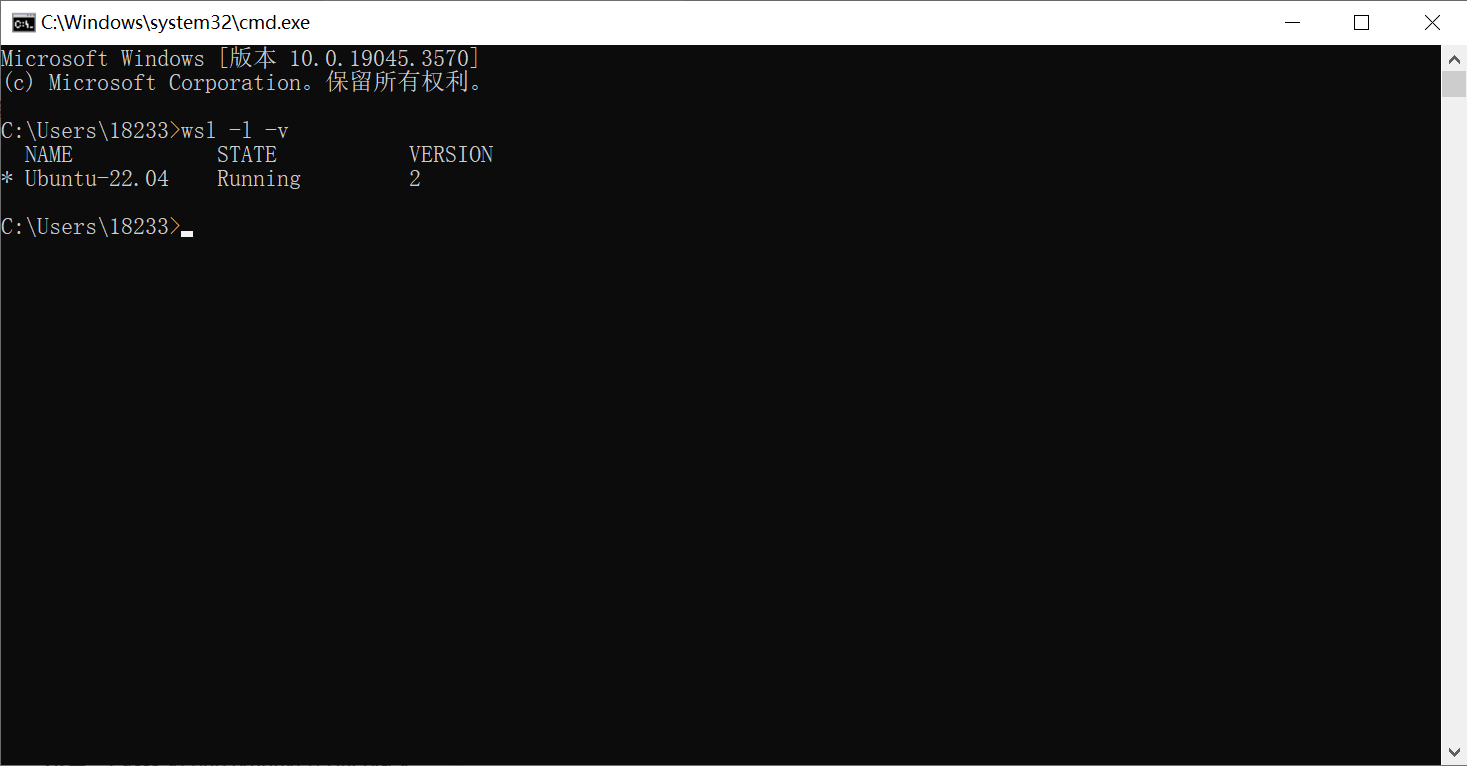
\includegraphics[width=16cm]{wsl-version.png}
        \caption{ubuntu22.04}
        \label{pic7}
\end{figure}

\newpage

    \item 安装annaconda
\begin{figure}[htp]
        \centering
        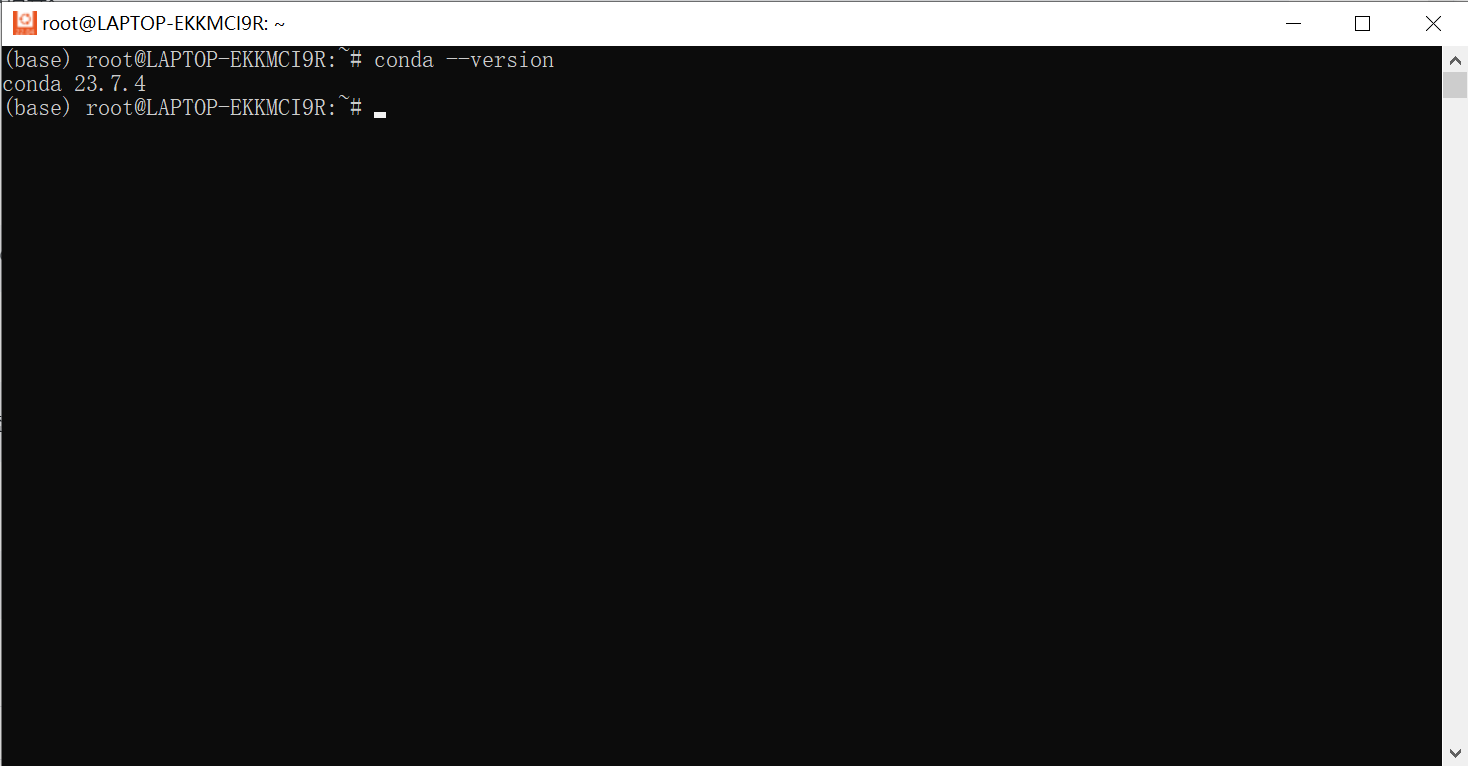
\includegraphics[width=16cm]{conda版本.png}
        \caption{conda23.7.4}
        \label{pic7}
\end{figure}

\newpage
    \item 下载源代码  git clone --depth 1 https://github.com/zjunlp/PromptKG.git
\begin{figure}[htp]
        \centering
        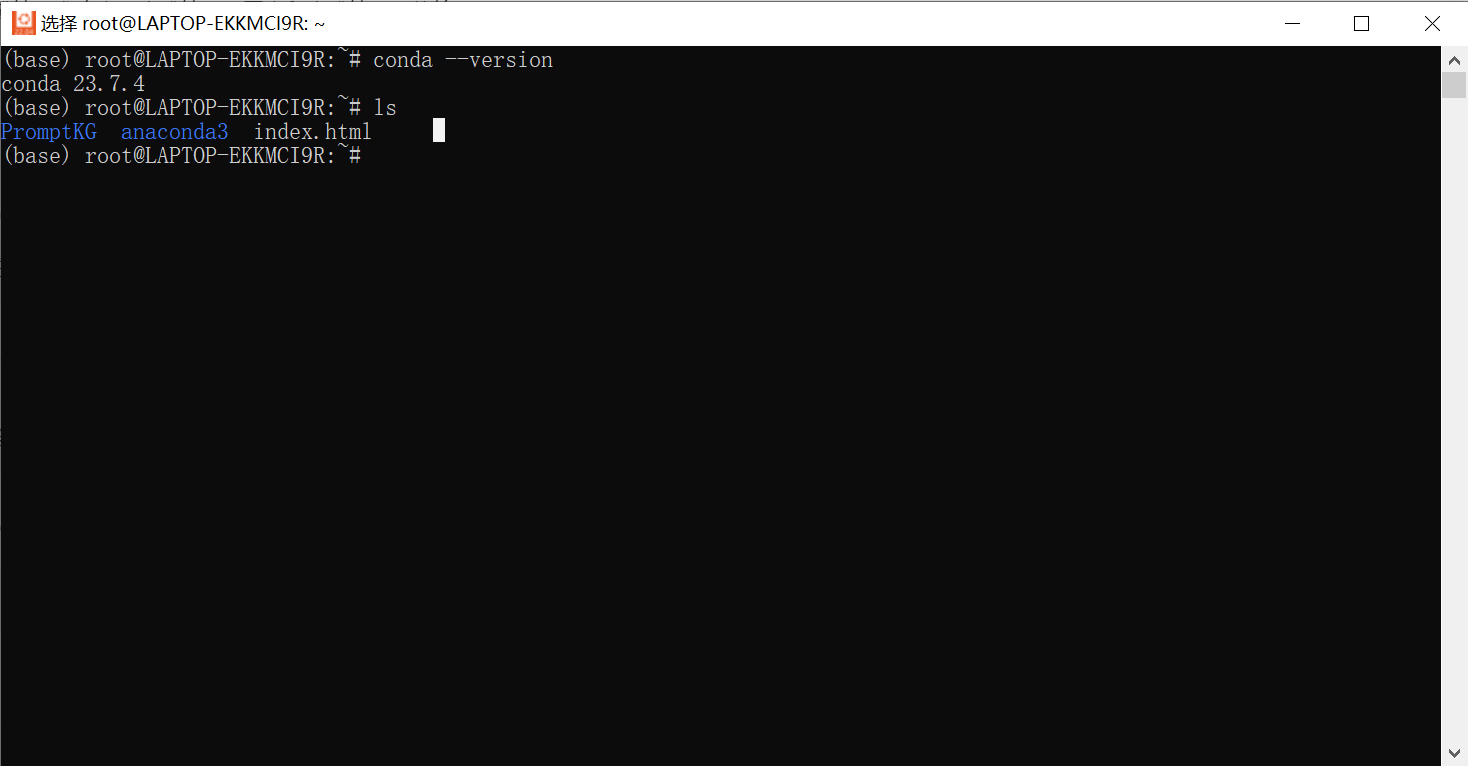
\includegraphics[width=16cm]{代码下载.png}
        \caption{}
        \label{pic7}
\end{figure}

\newpage
    \item 创建虚拟环境 conda create -n genkgc python=3.8 并激活 (conda activate genkgc)
\begin{figure}[htp]
        \centering
        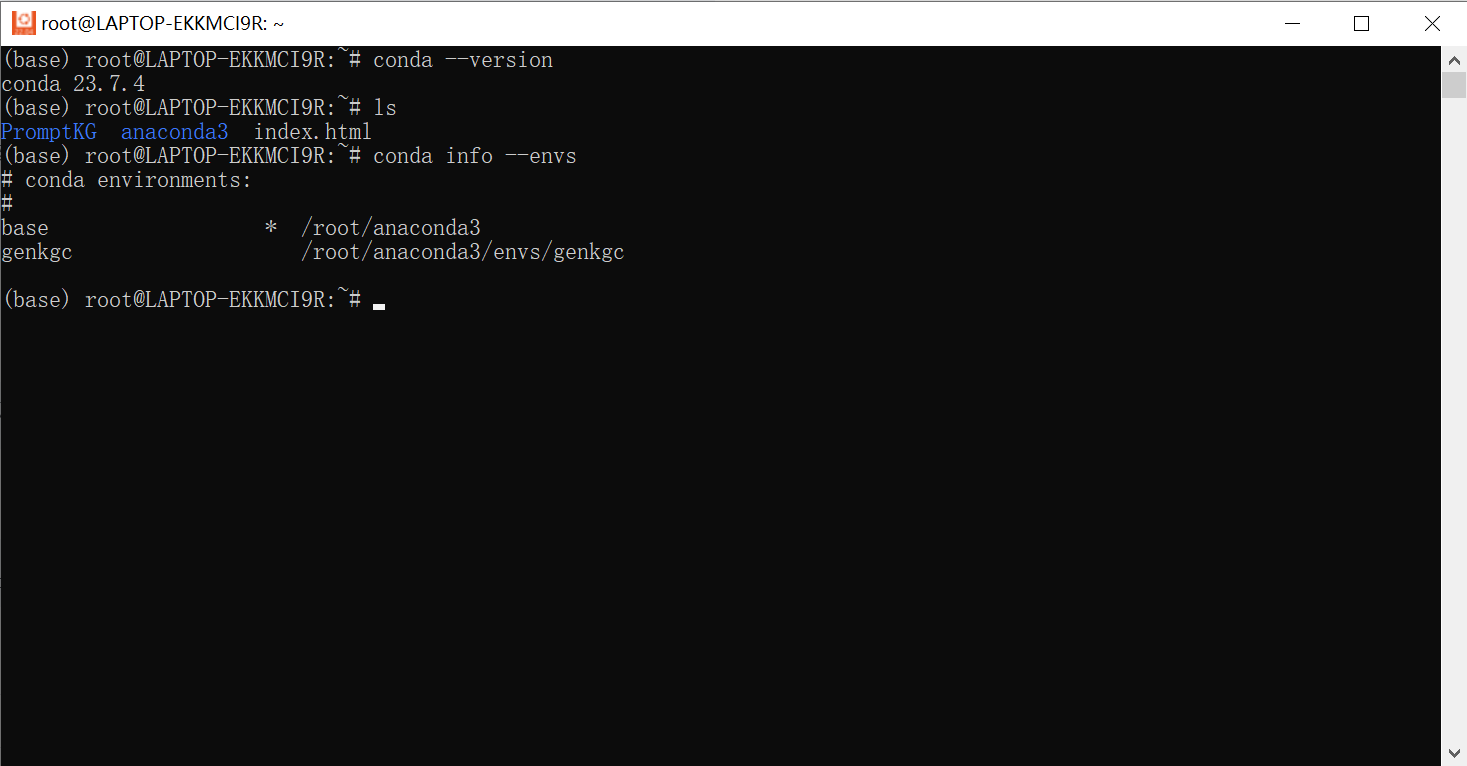
\includegraphics[width=16cm]{虚拟环境.png}
        \caption{}
        \label{pic7}
\end{figure}

\newpage
    \item 进入目录 (cd PrompKG/research/GenKGC)下载依赖 (pip install -r requirements.txt)
\begin{figure}[htp]
        \centering
        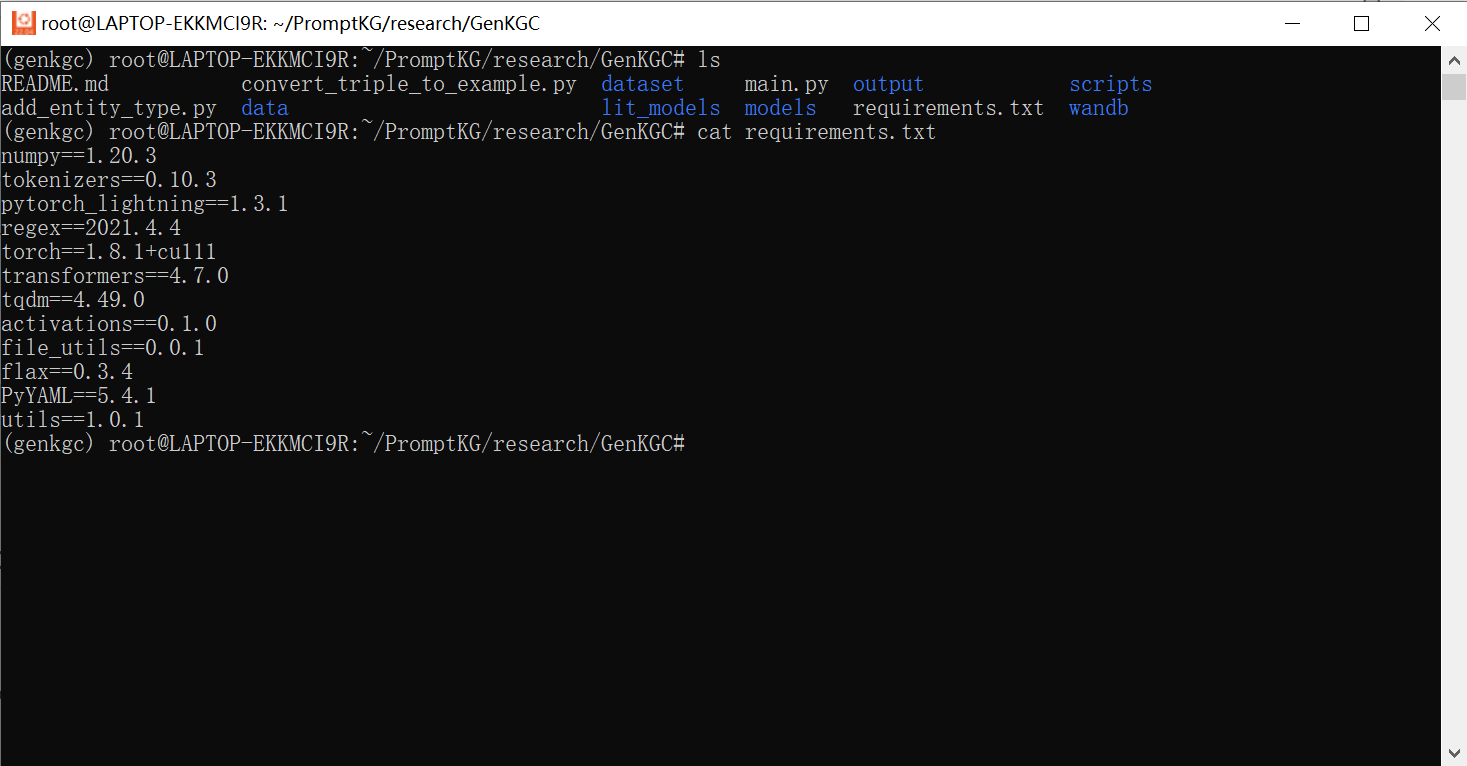
\includegraphics[width=16cm]{进入路径.png}
        \caption{cat requirements.txt}
        \label{pic7}
\end{figure}
    \item pip安装的所有包
\begin{figure}[htp]
        \centering
        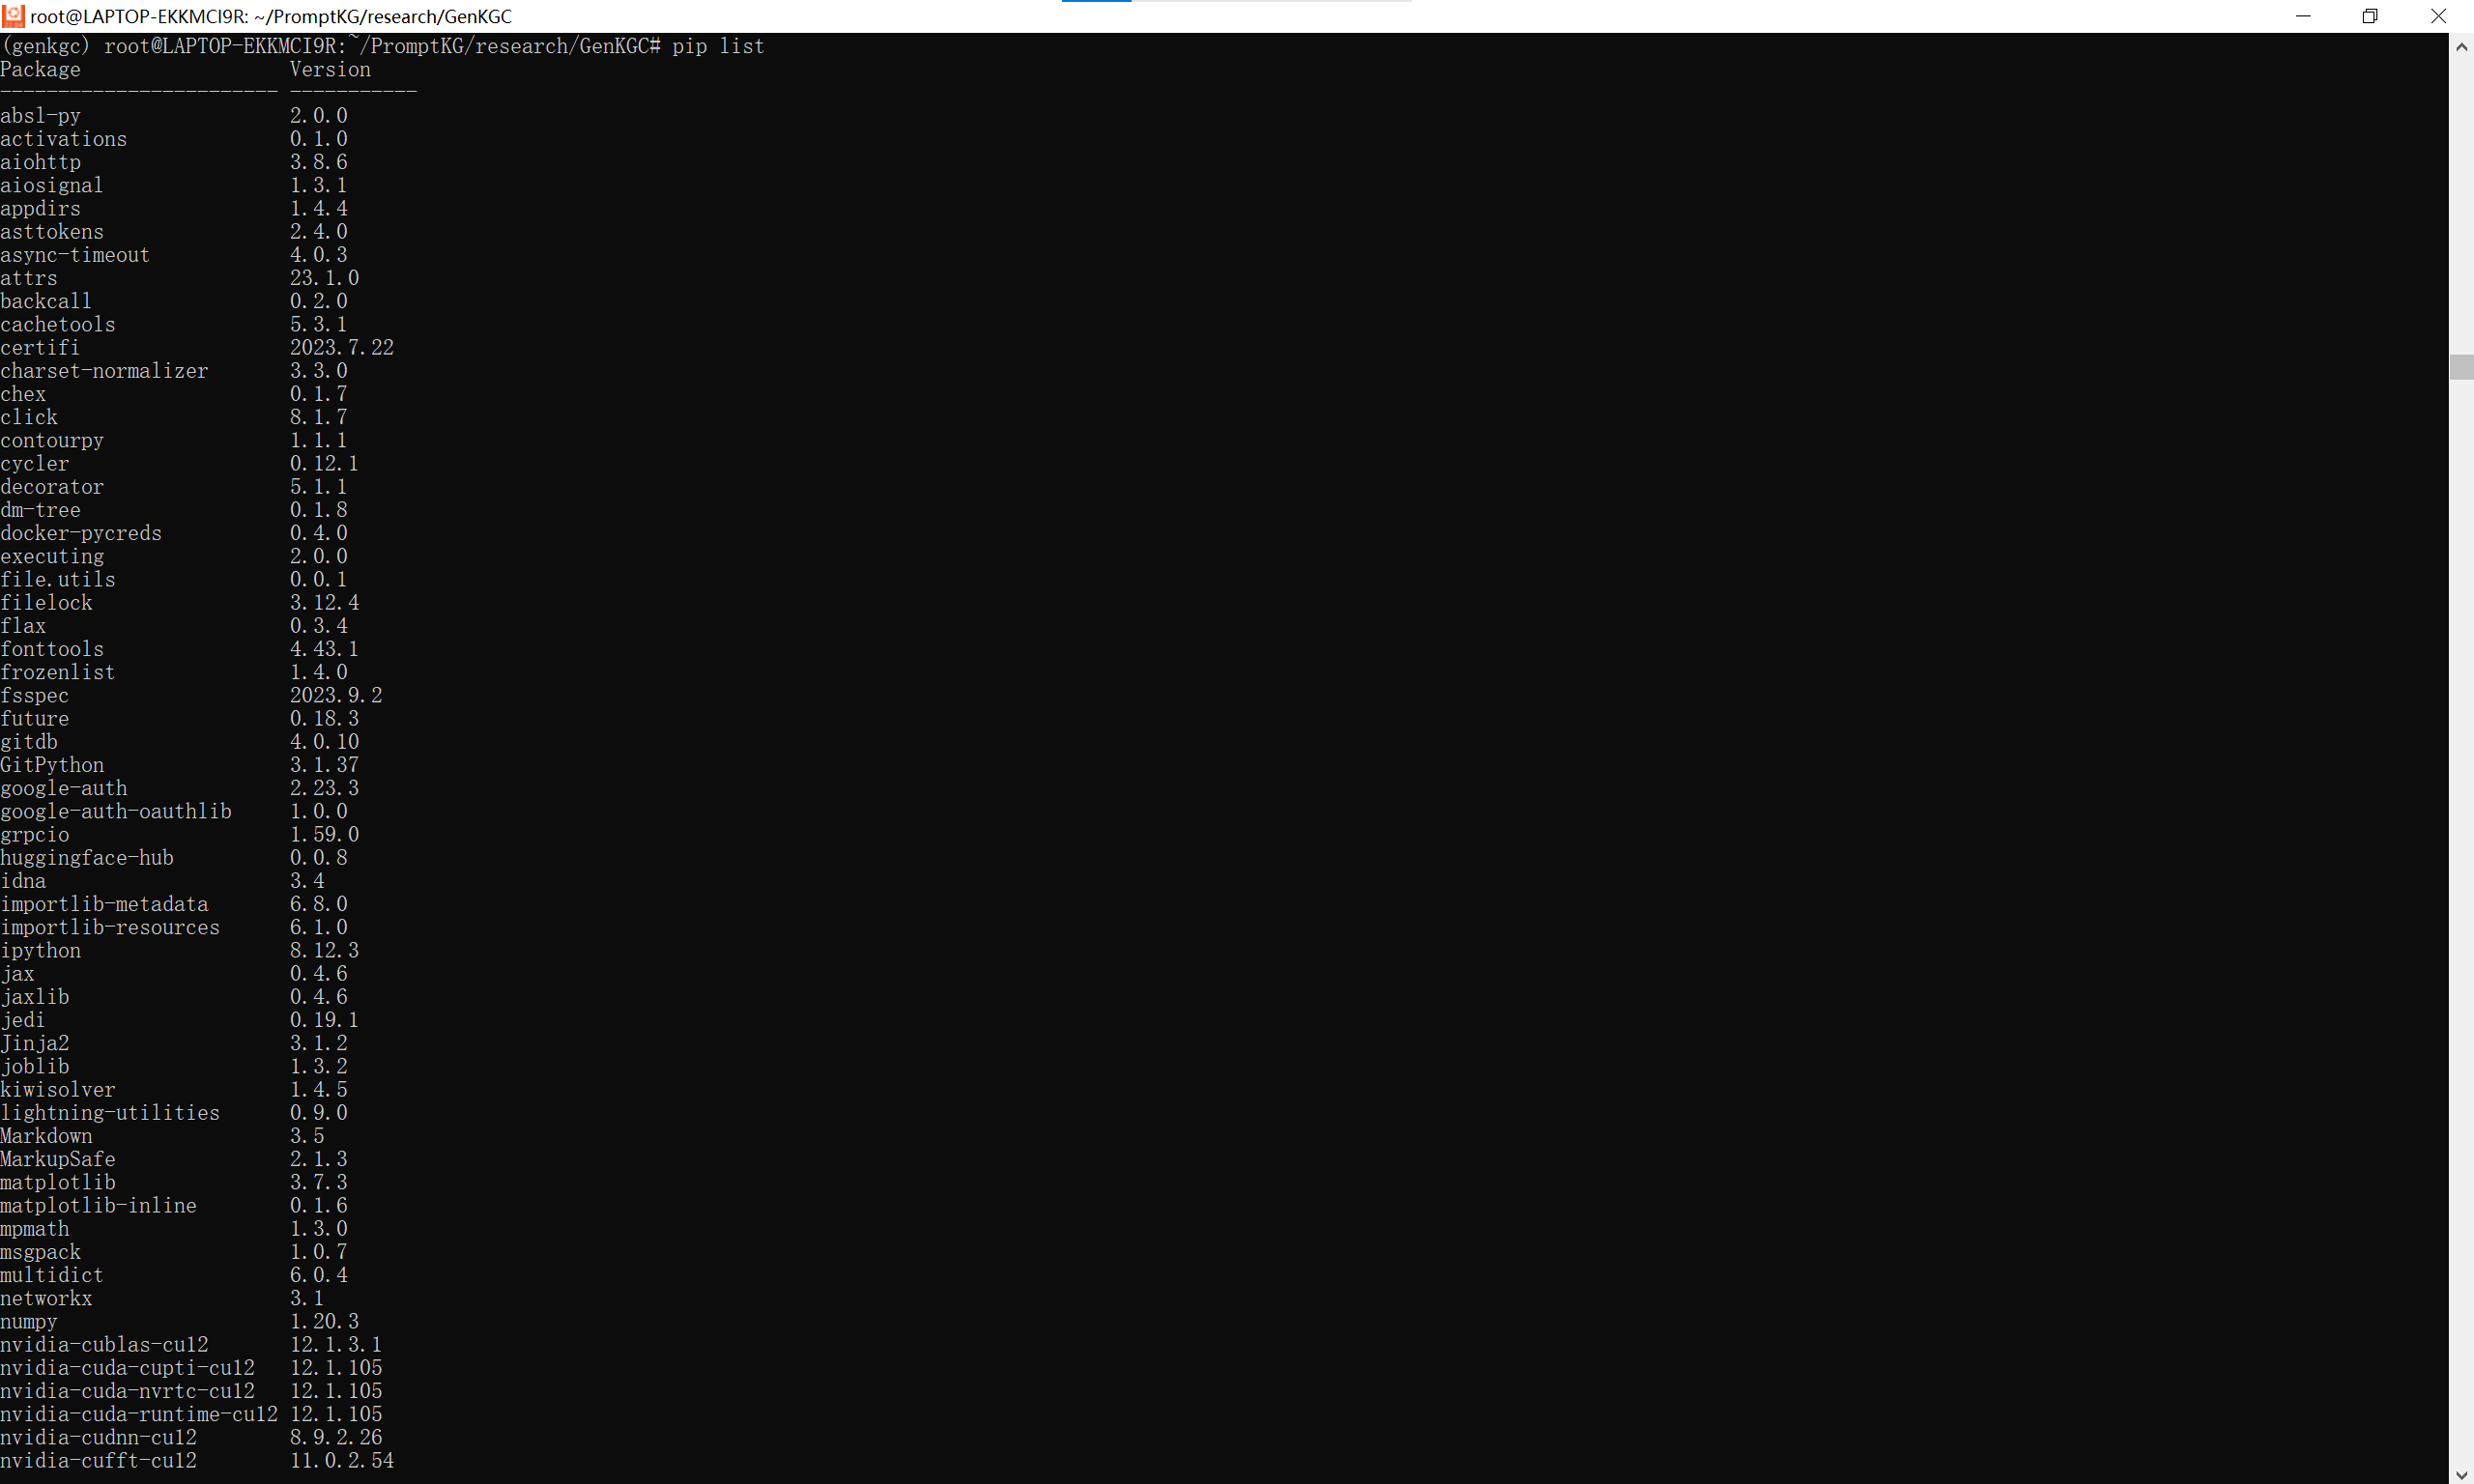
\includegraphics[width=14cm]{包1.png}
        \caption{pip list}
        \label{pic7}
\end{figure}
\begin{figure}[htp]
        \centering
        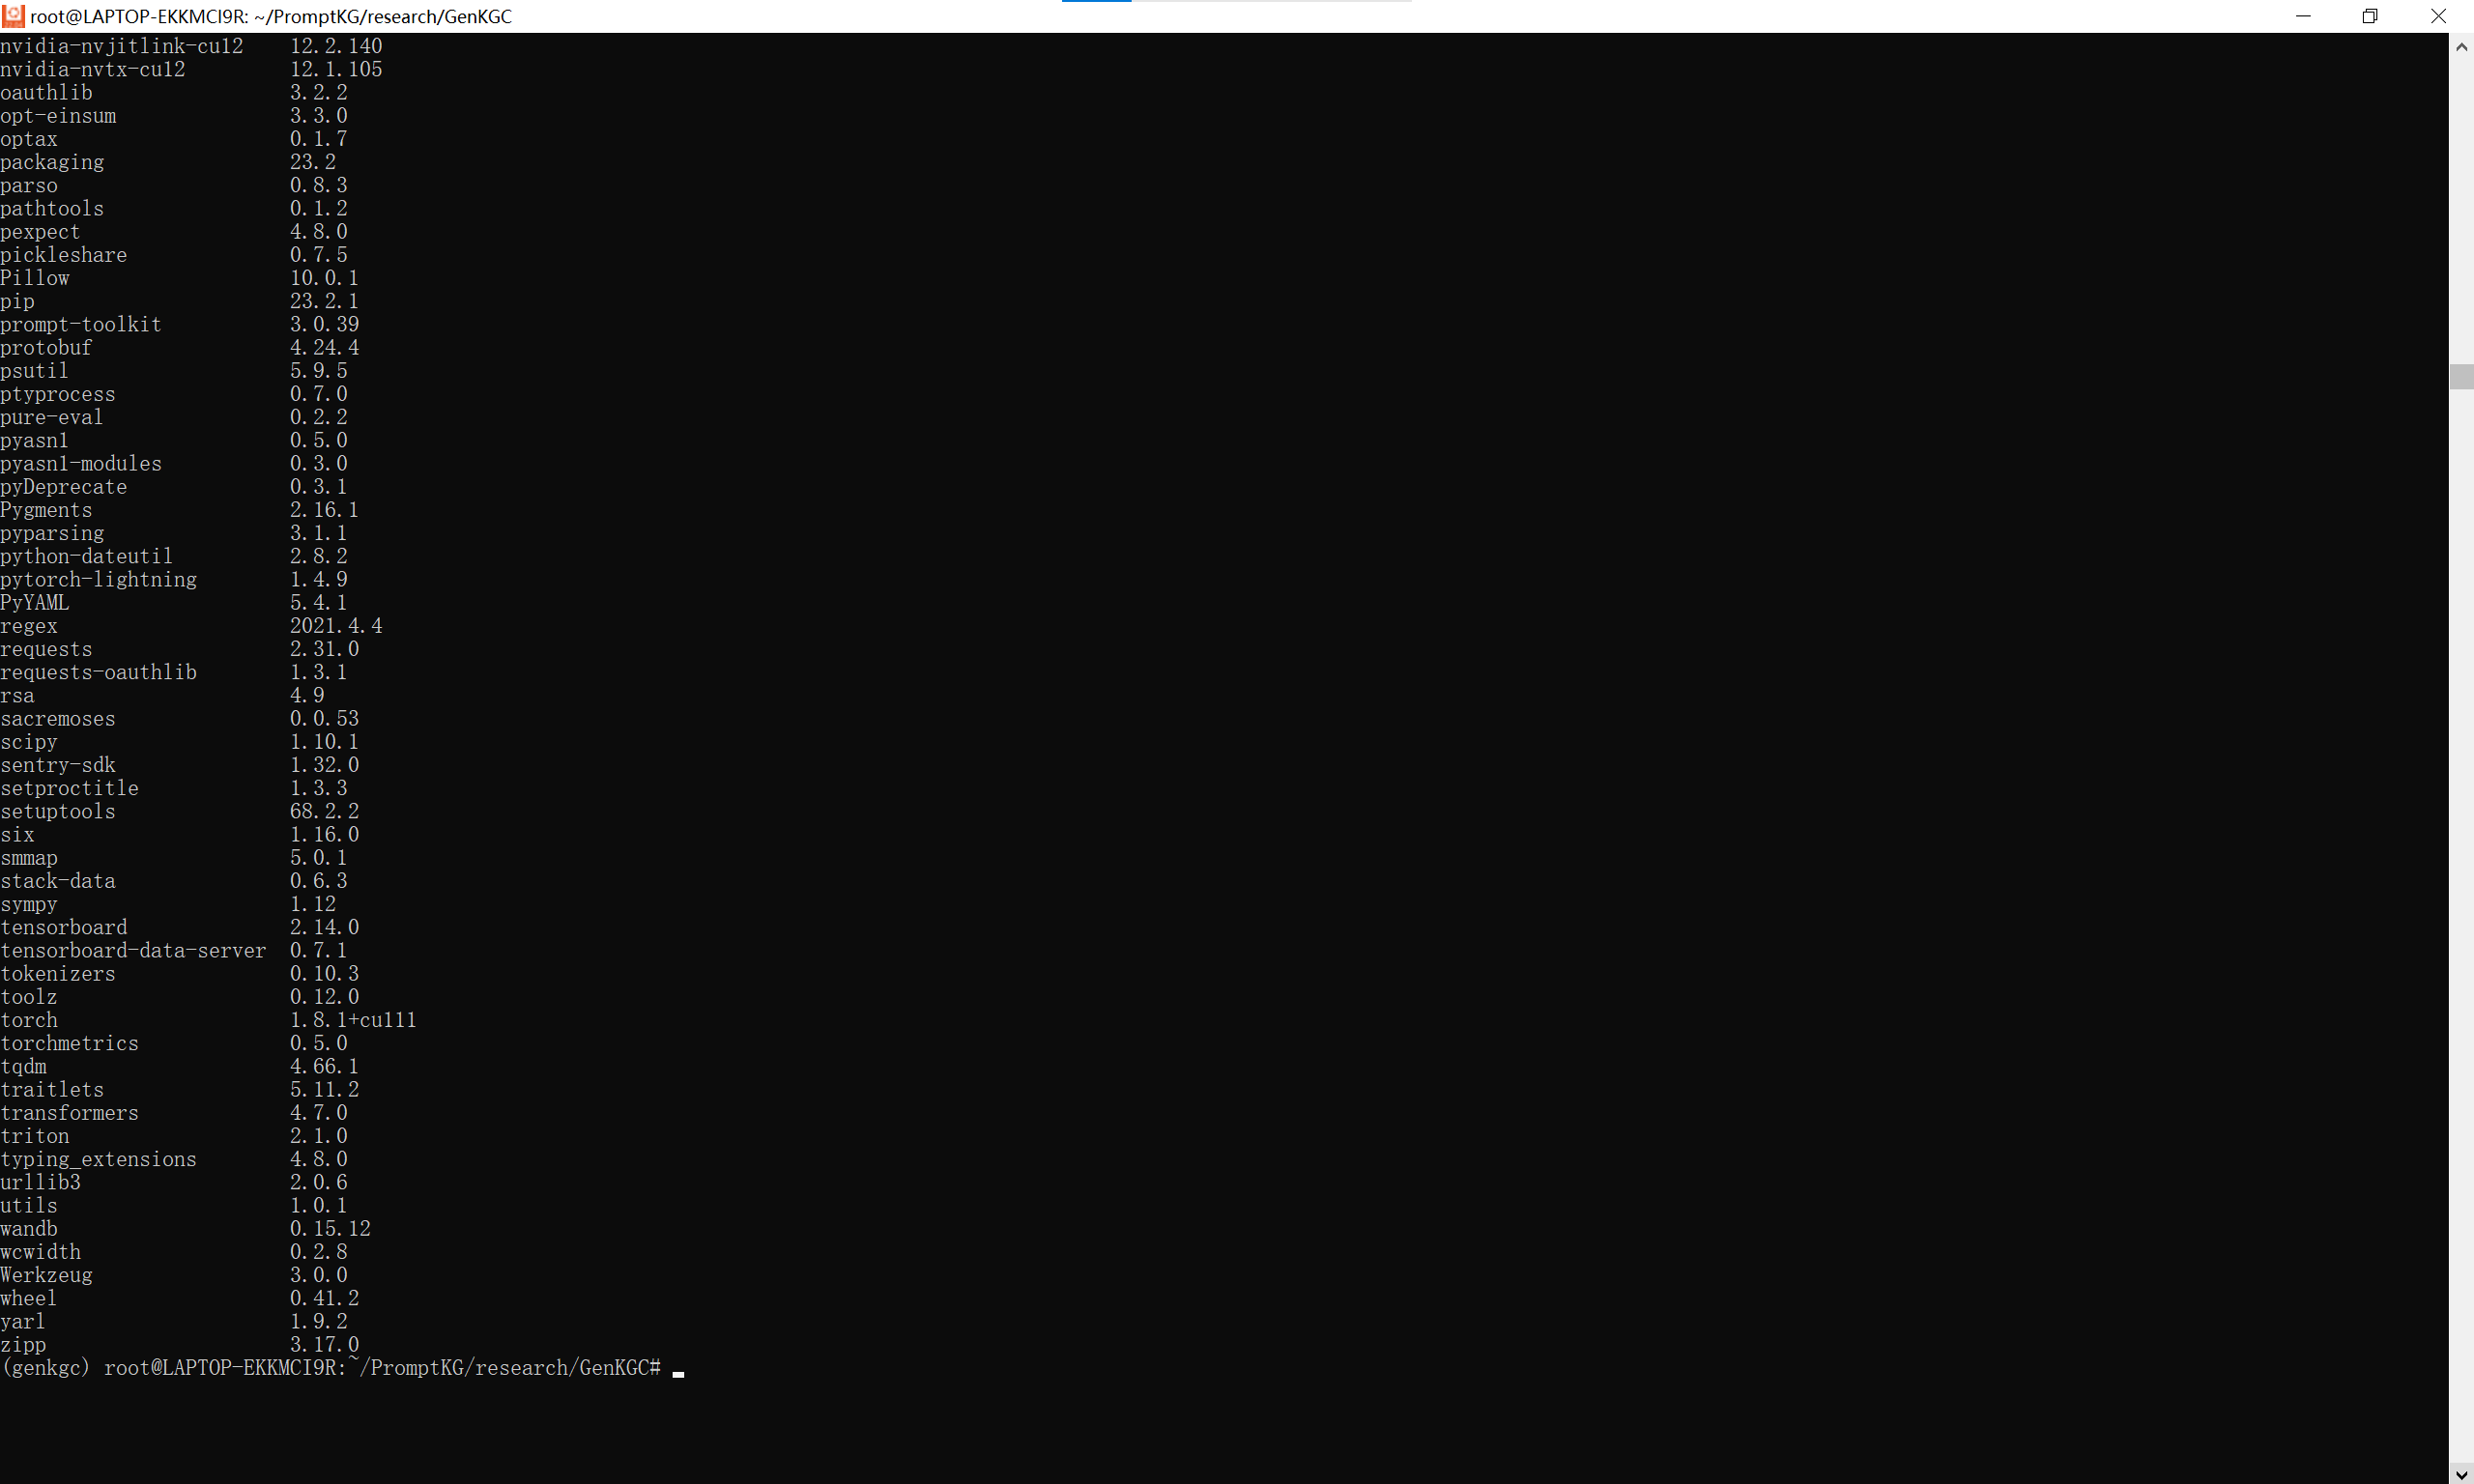
\includegraphics[width=14cm]{包2.png}
        \caption{pip list}
        \label{pic7}
\end{figure}

\newpage
    \item 下载数据集 git clone https://github.com/OpenBGBenchmark/OpenBG500.git
\begin{figure}[htp]
        \centering
        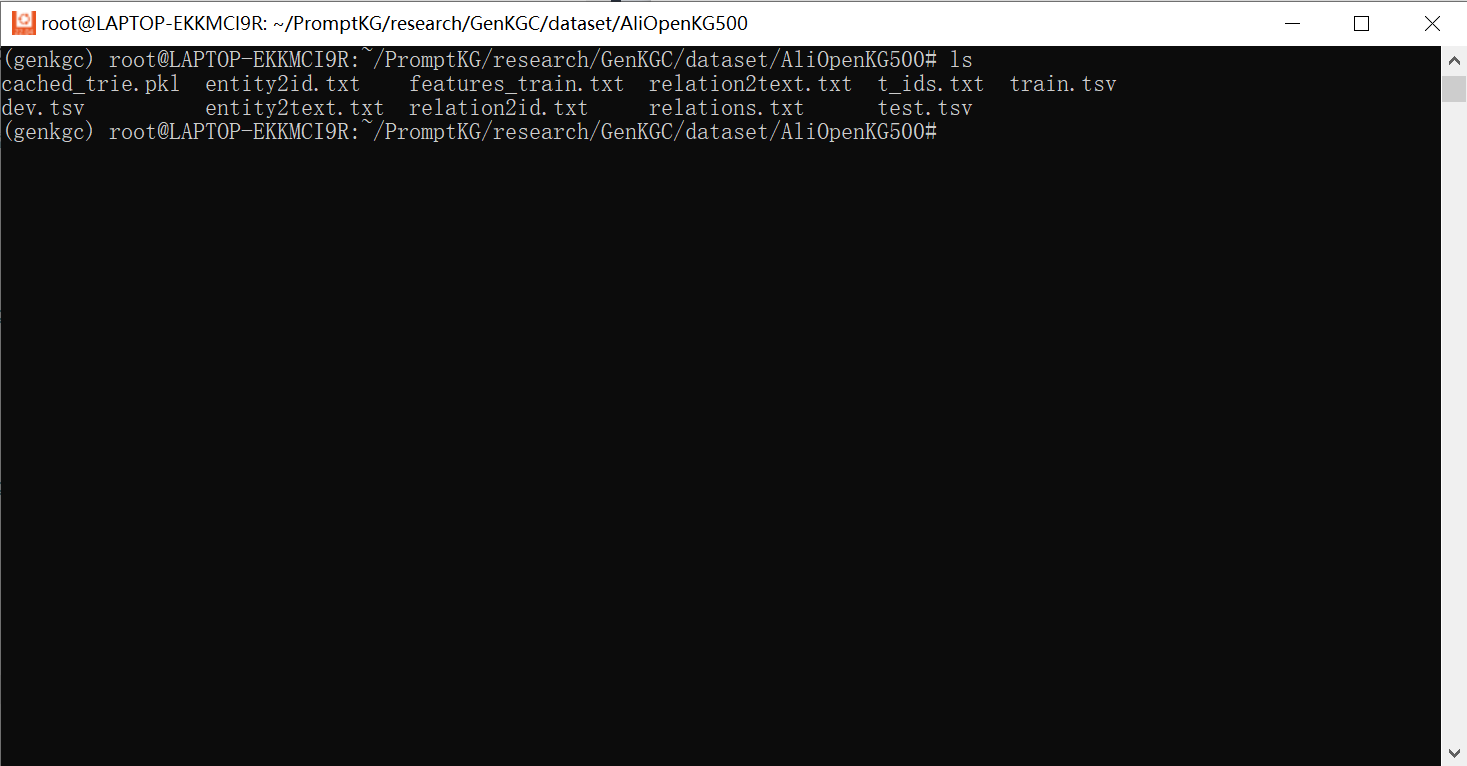
\includegraphics[width=16cm]{数据集.png}
        \caption{}
        \label{pic7}
\end{figure}
\newpage

    \item 运行代码 ./scripts/openbg.sh
\begin{figure}[htp]
        \centering
        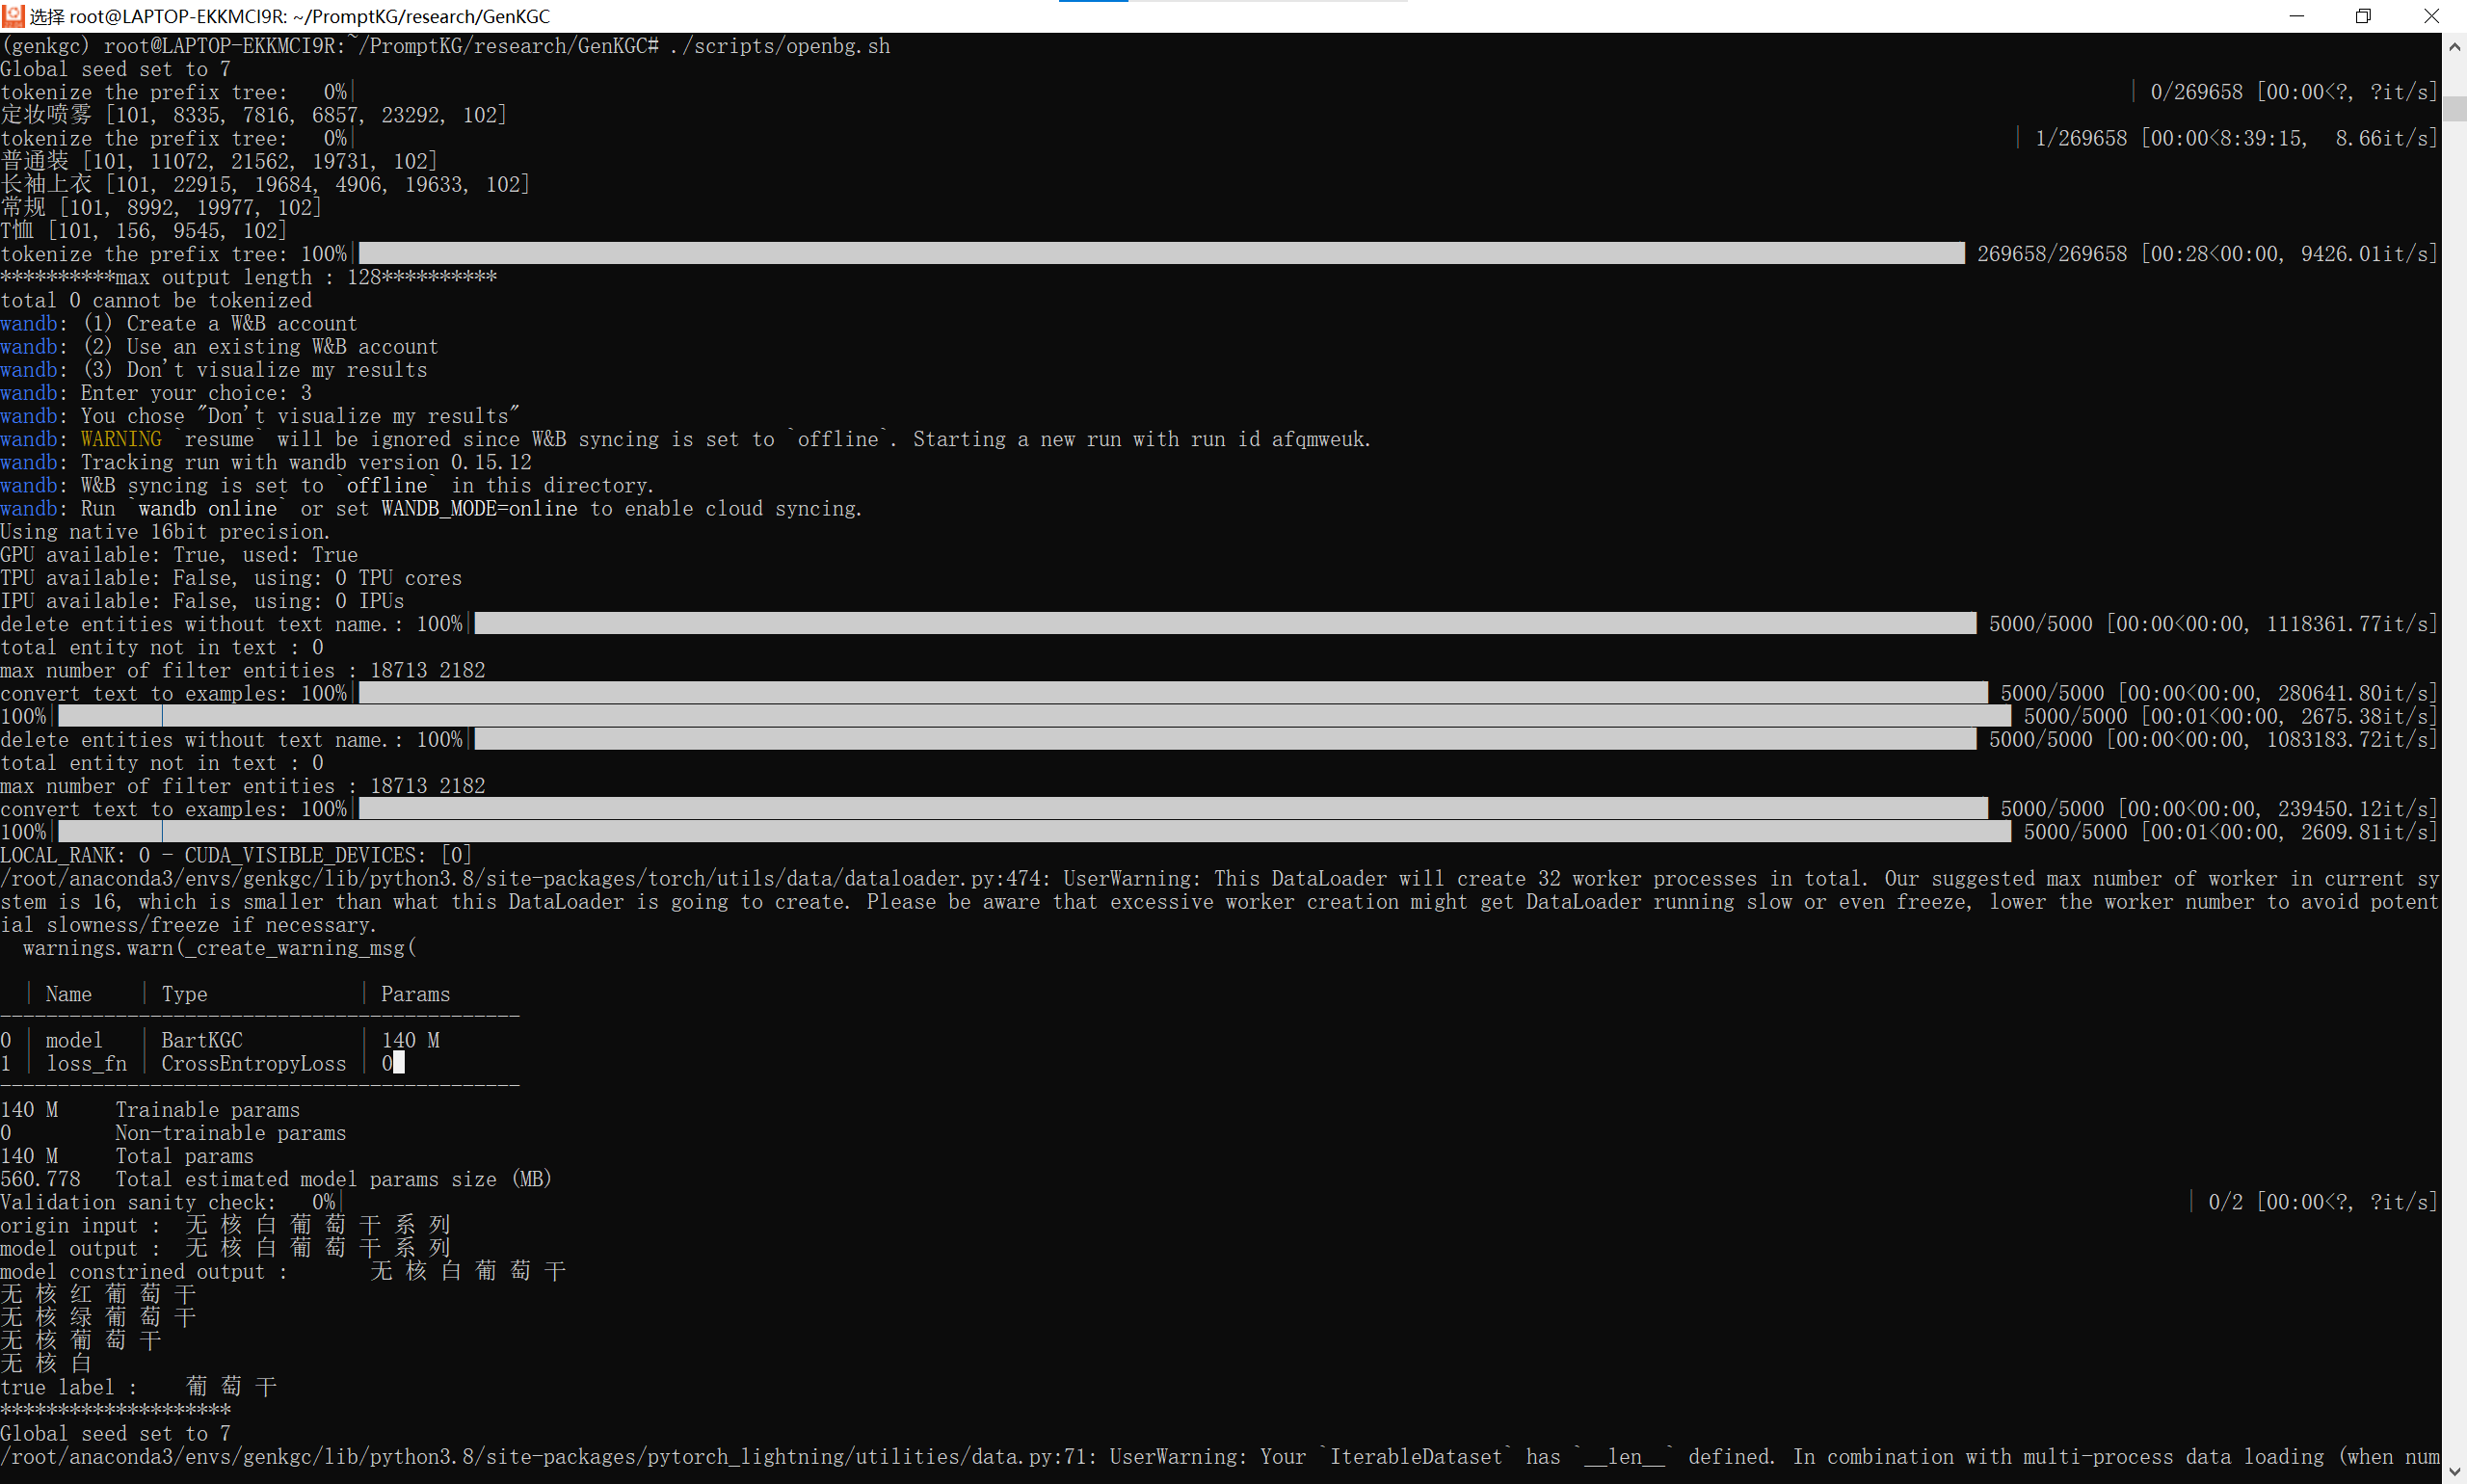
\includegraphics[width=16cm]{run.png}
        \caption{}
        \label{pic7}
\end{figure}
\begin{figure}[htp]
        \centering
        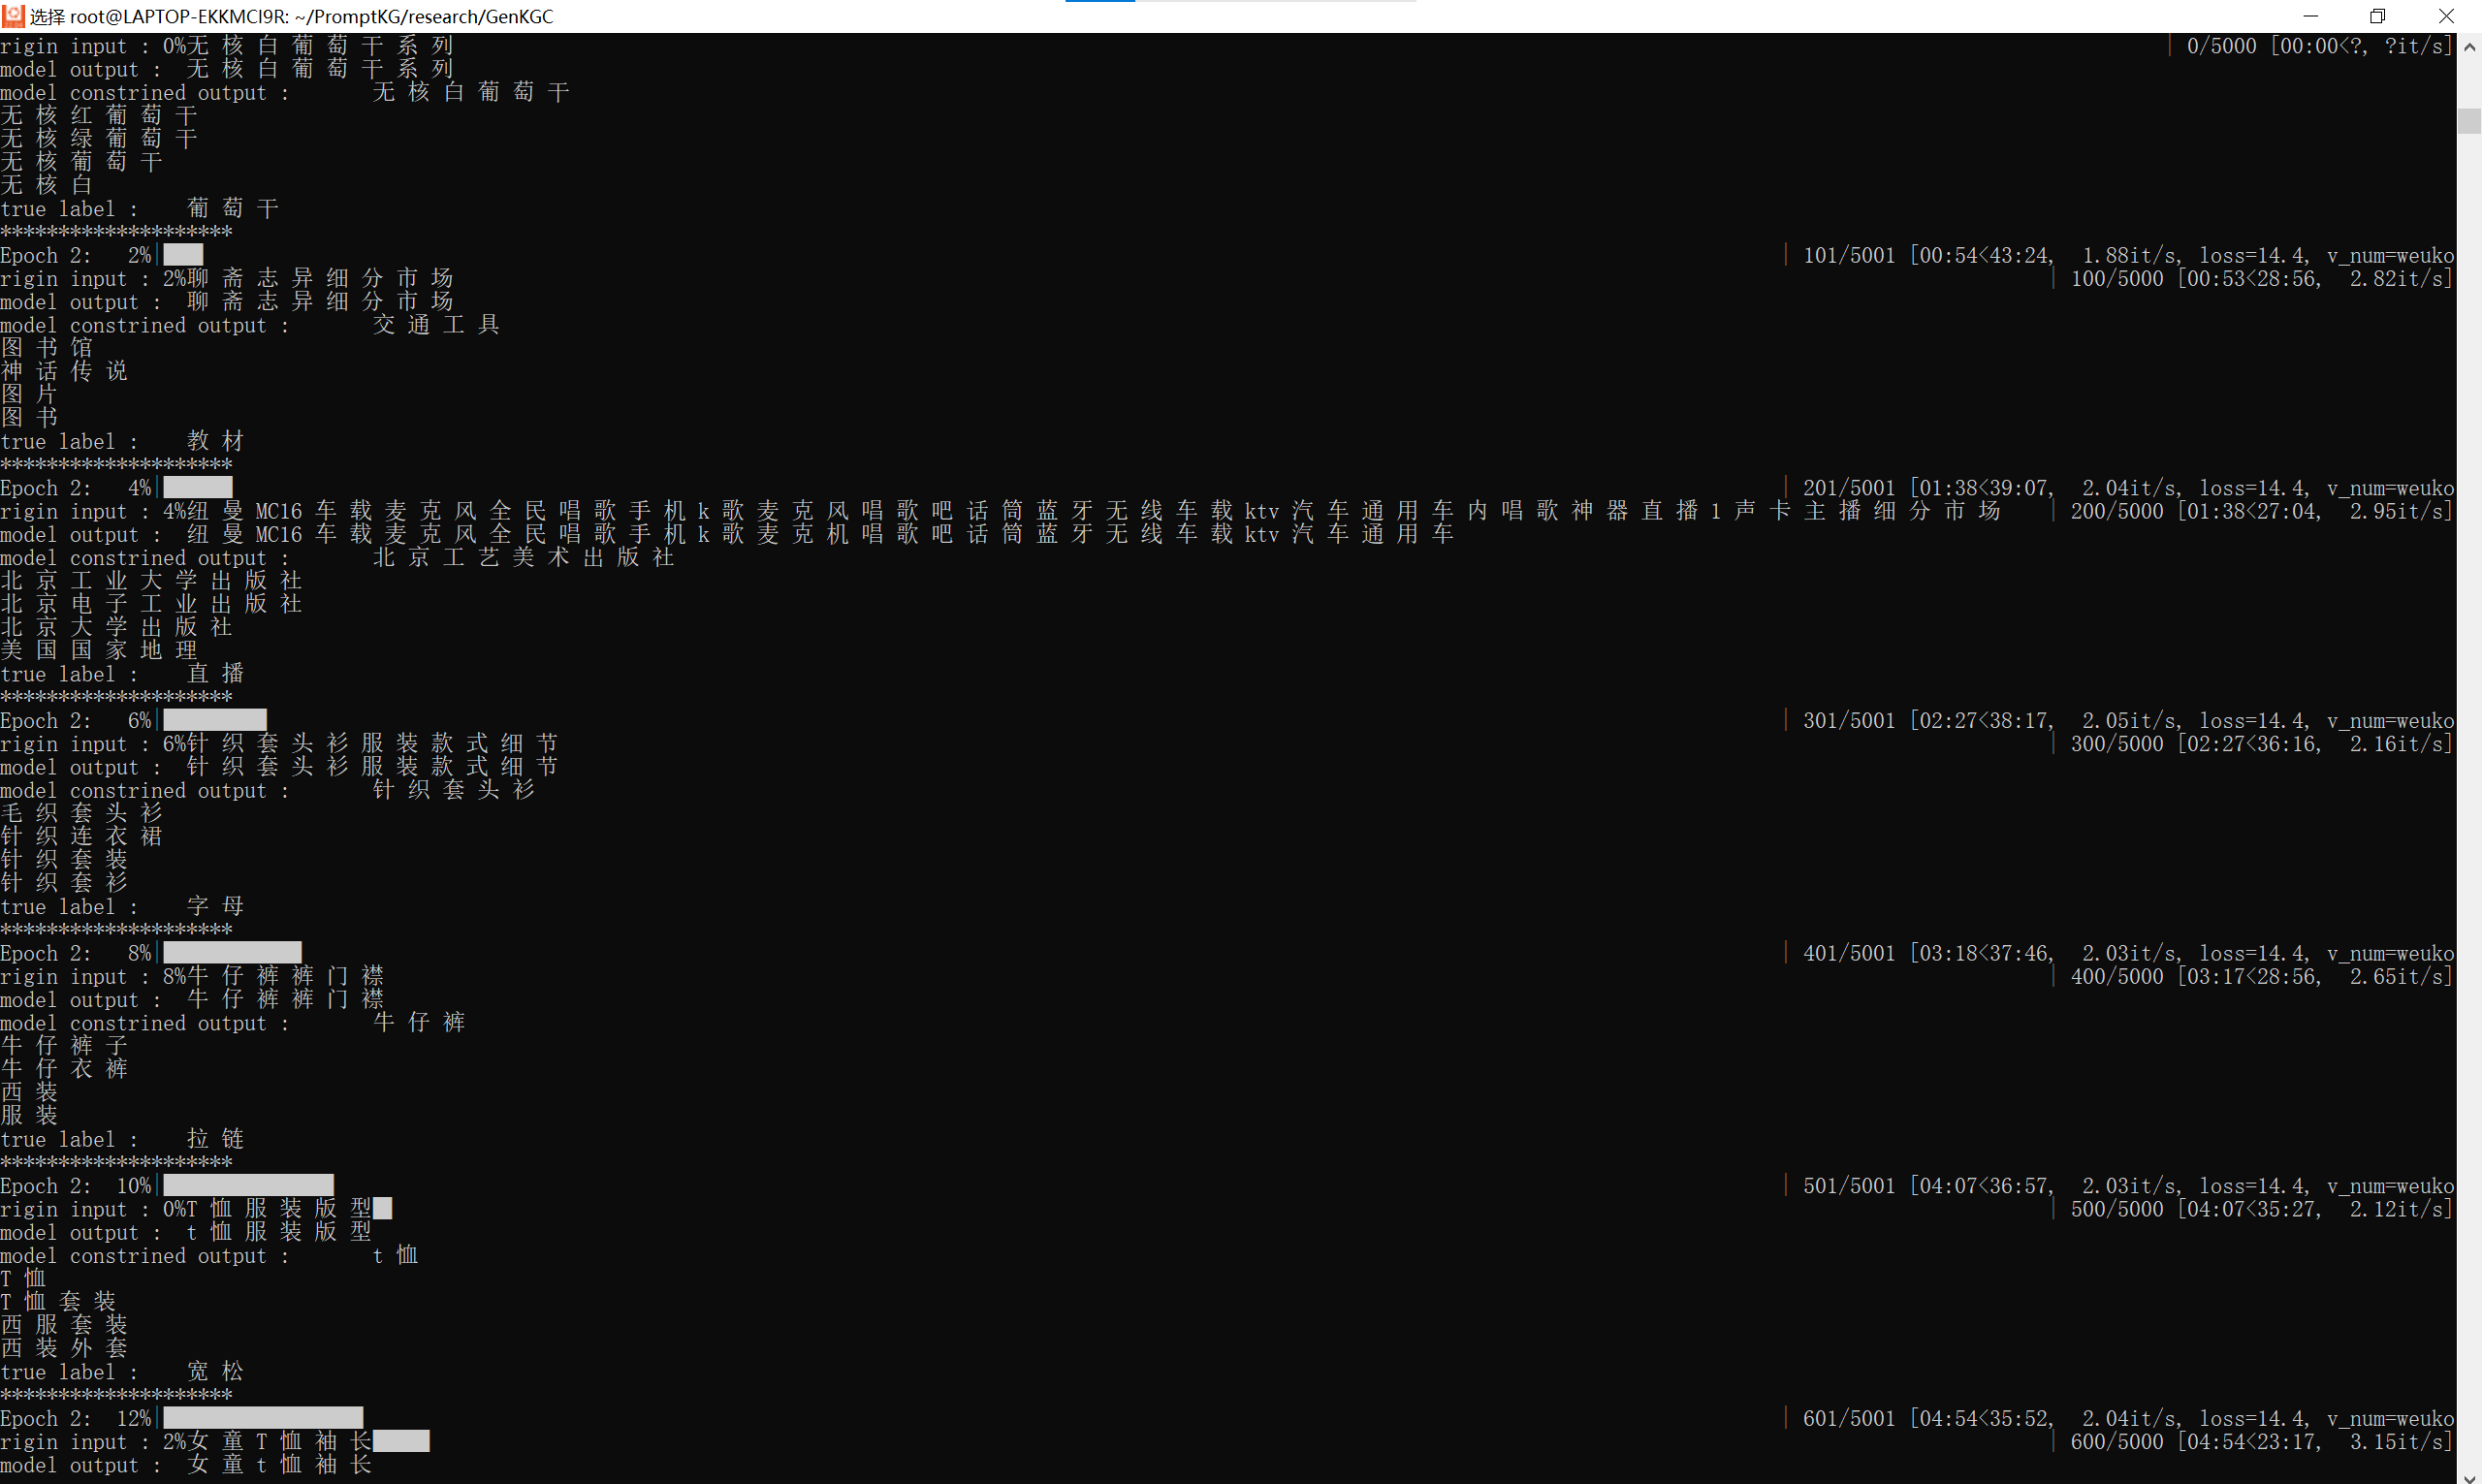
\includegraphics[width=16cm]{过程.png}
        \caption{}
        \label{pic7}
\end{figure} 
    
    \item 运行过程和结果
\begin{figure}[htp]
    \centering
    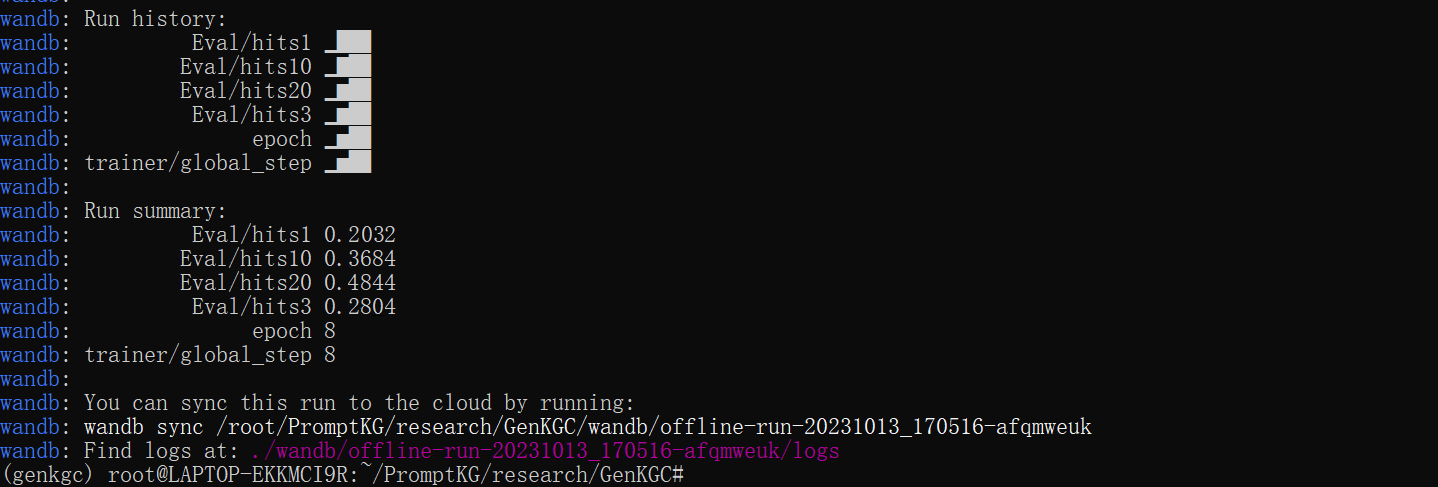
\includegraphics[width=16cm]{最终结果.png}
    \caption{}
    \label{pic7}
\end{figure}
\end{enumerate}
\end{document}
